%%%%%%%%%%%%%%%%%%%%%%%%%%%%%%%%%%%%%%%%%%%%%%%%%%%%%%%%%%%%%%%%%%%%%%%%%%%%%%%
%%%%%%% Customary 5-part intro explaining:
%%%%%%% Context, problem, prior work, insight and solution
%%%%%%%%%%%%%%%%%%%%%%%%%%%%%%%%%%%%%%%%%%%%%%%%%%%%%%%%%%%%%%%%%%%%%%%%%%%%%%%

% Context, computers are running ever increasing code bases, which are impossible to definitively verify
% and which are getting executed in shared environments all the time.
% Computer systems and computing environments have significantly evolved over time.
% \begin{itemize}
%   \item The complexity and scale of computing systems has increased exponentially for decades. 
%   \item The scale of modern systems allows, and also relies on, a large degree of sharing. 
%   \item The degree of code sharing has changed dramatically, 
%         from 
%         code written by individual tech-savvy developers and run on their personal machines
%         to 
%         code fully written and distributed by corporations and run by users on their personal machines
%         to
%         code written and distributed by a large variety of sources, and implicitly run in shared environments
%         by even unwitting users on personal machines.
%   \item Large amount of shared code cannot be vetted even by large corporations (e.g., popular libraries)
%   \item Shared code gets distributed by avenues with low checks or measures (e.g., package managers like crate, npm)
%   \item Browsers fetch and execute code on-demand from an infinitely varying set of sources.
%   \item Consequently, modern systems include a wider range of trust relationships compared to traditional systems.
% \end{itemize}
The computing landscape is one of rapidly growing software and hardware
complexity.
Modern computing systems inherit many of the abstractions and interfaces
developed at the inception of personal computing and mainframe servers,
but face a very different computing environment.
The complexity and scale of computing systems have increased 
exponentially over the decades, far outscaling the ability for developers to 
exhaustively test and verify their systems, leading to an abundance of bugs.
Popular software runs hundreds of millions of lines of source code, with
millions of lines worth of changes every year.
Linux, a widely-used operating system, itself currently accounts for
23 million lines of code, roughly increasing 20x since the turn of the
millennium.
Transistor counts for processors have roughly followed Moore's law for
the last 50 years, and a modern Apple M2 chip has more than a $10^{11}$
transistors compared to the $10^{4}$ transistors of the Motorola 68k processor
from 1979.
This scaling in complexity relies on, and also enables, pervasive code
sharing.
A web browser (e.g., Firefox) along with the underlying operating 
system (e.g., Linux) accounts for hundreds of millions of lines of code
including
\begin{itemize}
      % this point is meant to demonstrate the somewhat lack of formal structure
      % in Linux development. 
      % Individual devs are allowed to contribute their own improvements, 
      % alongside improvements planned centrally by Linus, maintainers and co.
      \item mainline kernel code written by a informal melange of developers
            distributed across the globe with varying 
            industrial/academic/governmental/individual affiliation,
      % fragmentation of sources/developers
      \item numerous device drivers written by the respective hardware 
            vendors,
      % absolute fragmentation of library development. popular libs developed
      % independently, and were incrementally adopted based on popularity
      \item shared libraries and modules developed independently and 
            written in a plethora of languages,
      % again, fragmentation of sources, but particularly on lack of trust
      \item code from websites, often embedding other pages,
            written by their respective web developers.
\end{itemize}
Modern systems need to consider the threat of bugs in shared code
compromising their security, and implement the necessary mitigations.
For example, a web developer must account for the threat that any of the
thousands of JavaScript packages their code depends on might be malicious,
currently or in the future.
The security of computing is reliant on the security properties at the 
interfaces between components (trusted and untrusted).
The abstractions and interfaces at the core of computer systems need to
enable systems to face up to today's security challenges.
% See this example:
% https://therecord.media/malware-found-in-npm-package-with-millions-of-weekly-downloads


% The core problem: mismatch between interface design and modern computing trust relations
% Modern systems are implemented on legacy interfaces, incurring security or performance limitations.
% \begin{itemize}
%   \item modern systems continue to rely extensively on legacy interfaces. 
%   Examples  of these interfaces include the ISA interface and OS system call interface, both of which largely resemble systems from 20-40 years back.
%   For example, the virtual memory definition of traditional ISAs focus on isolating different virtual address spaces from each other, whereas modern systems mix code from various untrusted sources within the same address space.
%   \item Interfaces might lack the expressivity to express modern trust relations (virtual memory)
%   \item Interfaces might include implicit assumptions, including ones not noticed by the developers of the interface, which may be wilfully or unknowingly violated by malicious or buggy code.
% \end{itemize}
% Problems with two specific interfaces are tackled by this thesis.
% \begin{itemize}
%   \item The OS interface to userspace lacks protection against concurrent modification by userspace. 
%         A contributing factor to this problem could be the relative absence of concurrency, and absolute 
%         lack of parallelism when modern operating systems were conceived.
%   \item The ISA interface for virtual memory contains a single permission for any address, for all code
%         executing within that address space.
%         This design was sufficient when programs trusted all of their code, moreso since most computers 
%         ran code entirely designed and written by one corporation.
%         The relative infancy of the internet meant very limited code sharing, and only among developers when
%         at all.
% \end{itemize}
While computing systems have evolved significantly, interfaces between many 
parts of this system have remained relatively unchanged.
The designs of these interfaces reflect the requirements and threat landscape
from their respective design periods, but fail to adequately address modern
needs.
Linux, for example, started development in the 1990s and is heavily inspired
by Unix, initially developed in the 1960s-70s.
The Linux kernel system call interface is cognizant of the threat of attacks
or faults from untrusted userspace compromising the kernel, reflecting the
contemporary shared use of mainframes running applications for a limited
set of known users.
System calls, therefore, typically check the validity of arguments passed
from userspace.
However, computing and the associated threat vectors developed over the
past 30 years, rendering Linux' original system call interface dated.
Systems running untrusted code have become ubiquitous 
(cloud computing, applications distributed over the internet, and
sandboxed code within browsers) necessitating stronger isolation between
system users, and even isolation between parts of the same application.
These systems 
One consequence of the dated designs of key interfaces is that these interfaces 
might not adequately mitigate threats
that have arisen or worsened after the design of the interface.
Since the 1990s, computing has evolved to support increased concurrency and true 
parallelism, with the rise in popularity of multicore CPUs and multi-threaded 
programs.
For system call arguments stored in user memory and passed by reference,
this evolution has enabled data races if the user program
modifies the arguments from a second thread while the kernel executes
a system call from one thread.
This trend extends to other interfaces with widespread usage.
The C programming language, dating back to the 1970s, remains in popular use
despite the lack of memory safety by default.
The rise of the internet and corresponding emergence of cyber warfare has
exacerbated the effects malicious exploitation of memory safety bugs, 
leading to major vulnerabilities 
(e.g., Heartbleed~\cite{cve20140160}, GHOST~\cite{cve20150235} and NetUSB~\cite{cve20153036}).
A second consequence is that interfaces might not provide the correct
abstractions to efficiently support designs that reflect
trust relations within parts of modern applications.
For example, the dominant abstraction for isolation within userspace code
is a process, and different applications typically execute in different 
processes to isolate applications from bugs in other applications.
The process virtual memory interface is supported by hardware enforced
page table permissions across major commercial instruction set architectures
(x86, SPARC, ARM) developed across the 1970s and 1980s.
Process isolation is well suited to the historical state of software
development where software vendors wrote their own applications with limited
code sharing between vendors.
Processes isolated code for one application, from one software vendor,
from other applications, from other software vendors or for another user.
With more code within applications originating from third-party developers
and less trust in code run within a single process, intra-process isolation
has become crucial.
Security-critical programs, like browsers, microservices and microkernel
operating systems (OSs), refactored to enforce intra-application isolation 
using processes are limited by the high overheads of this abstraction, and 
only support coarse-grained isolation to cap 
performance overheads~\cite{ChakraCore, wxexclusionfirefox,barth2008security}.


% Prior work around fixing abstractions or introducing new ones
% Recent work has started tackling this problem at various levels. 
% \begin{itemize}
%   \item Papers have tried to remove this implicit assumption from the kernel by attempting to find and 
%         refactor code vulnerable to userspace TOCTTOU, using methods based on static and dynamic analysis.
%         Limitations of existing works includes:
%         - protection only against known bugs, 
%         - detection of subset of bugs triggered by dybnamic analysis,
%         - other shortcomings described in the paper.
%   \item Mechanisms (research and production) have tried to introduce additional access control within an
%         address space to isolate parts of a program which do not trust each other.
%         However, these mechanisms continue to trade-off performance and security guarantees. 
%         - Some existing mechanisms offer a thin additional layer of security for very little overhead.
%         - Others provide more comprehensive protection, but at high cost.
%         A common contributing factor to higher costs is a reliance on more traditional abstractions.
%         Particularly, the OS is included in the TCB and tasked with implementing switching between
%         protection domains or compartments, assuring security at high cost.
% \end{itemize}
Recognizing emerging threats, key interfaces have gradually evolved, 
fixing bugs and introducing new defense features.
Most improvements tend to be incremental.
By adding a NX/XD bit to mark pages as non-executable, popular
processor architectures added support for Data Execution Prevention (DEP)
and prevented code injection exploiting buffer overflows.
Over the years, millions of commits have added various patches to Linux.
However, many improvements address individual bugs while failing to
comprehensively improve an interface's security.
Continuing industrial and academic efforts have proposed various 
improvements to improve the kernel-user boundary and add support for 
isolation within an application.
The security of operating system kernels is an area of active research, and 
many
methodologies have been proposed to fix the issue of data races at the system
call interface, primarily focussing on finding and fixing instances of this 
class of bugs.
One group of proposals leverage 
static analysis~\cite{dftinker, wang2017double, wang2019dftracker, deadline}
to comb through the 
kernel codebase looking for vulnerable double fetches.
These static analysis techniques have progressively improved
from matching code against known double-fetch bug patterns to
symbolic execution-based analyzers.
Alternative proposals
leverage dynamic analysis to detect instances of data races at 
runtime~\cite{jurczyk2013bochspwn, schwartzDECAF, wilhelm2016xenpwn}
by tracking kernel memory accesses while executing various common 
workloads (for e.g., booting up, running a browser, playing multimedia).
Eliminating the discovered data race bugs by fixing source code allows the
kernel to present a more secure interface, though the invulnerability to 
data races remains an informal assumption rather than a guarantee.
% schwartsDECAF has decaf - detection, dropit - mitigation.
Finally, a proposed mitigation~\cite{schwartzDECAF} repurposes a CPU-specific
feature
designed for accelerating database transactions to instead dynamically
detect user updates between kernel double fetches, rolling back the
system call execution to prevent exploitation.
Bug squashing techniques, however, are insufficient --- they can only fix
bugs found --- and both static and dynamic analysis are incomplete.
The significant churn in code further complicates the challenge, as every
change potentially introduces new double-fetch bugs.
The proposed mitigation is also inadequate, since the protection depends on
a vendor-specific feature which has since also been deprecated on newer
processors.
The system call interface requires a more principled and reliant
mitigation against data race attacks.
Similarly, while researchers and processor vendors continue to propose 
mechanisms for finer-grained isolation within a process' address space, 
these mechanisms vary in their design goals, and do not adequately
support widespread adoption of compartmentalization.
Mechanisms which prioritize backward compatibility with existing 
systems~\cite{LittonVE0BD16, HsuHEP16, HedayatiGJCSSM19Hodor, LeeSK18, DuHXZC19XPC}
introduce the security benefits of intra-address space isolation
but continue to suffer the consequences of other legacy design choices, 
such as expensive supervisor-mediated context switches.
Some mechanisms~\cite{ParkLXMK19, HedayatiGJCSSM19Hodor} trade off 
performance for security, either providing weaker security than processes
to provide better performance or making restrictive assumptions on
application use cases.
A common approach among researchers is to retrofit protections to vulnerable
interfaces abusing the side effects of unrelated mechanisms co-existing on
the systems, bringing immediate protection to certain systems at the cost
of a few fundamental shortcomings.
Researchers have applied this approach to both mitigate double-fetch
bugs~\cite{schwartzDECAF} using Intel TSX and to implement 
compartmentalization~\cite{HedayatiGJCSSM19Hodor,LeeSK18} using Intel VT-x.
This approach is limited by dependence on specific 
systems (using Intel CPUs, for example) and potentially
inhibits concurrently using applications requiring these features for their 
proper functioning.
Most importantly, such defense mechanisms lack principled design and 
resemble targeted protections rather than 
fundamental security guarantees baked into interface design.

% Insights: Problems with abstractions can be fixed. 
% Fixes might require principled changes to the interfaces, as either mitigations which preserve the
% interface but allow additional checks to be implemented, or as a redesign of the entire interface.
% In this thesis, we solve the two interfaces by:
% \begin{itemize}
%   \item We recognize that
%           TOCTTOU comes in the insight that devs make an implicit assummption.
%         System calls implicitly assume that their view of accessed user memory does not change
%         during the system call's lifetime. 
%         The kernel uses a well-defined software interface to access user memory. 
%         The clean separation of the access interface allow additional checks to assure that 
%         the implicit invariant is upheld.
%   \item The hardware is part of the TCB, and can be tasked with managing permissions for different
%         compartments, read from one two-D table.
% \end{itemize}
Security guarantees should inform the design of interfaces --- either by 
extending or redesigning interfaces.
% 
At the kernel-user interface, we see that data races require the kernel
to access the same argument in user memory at least twice, which
allows the user to modify the data in the meantime.
In fact, such bugs which are generally called double-fetch bugs 
commonly (but not exclusively)
manifest from the same usage pattern.
The kernel first loads arguments once to check their validity, then
loads them at a later time in order to use them.
This pattern earns these bugs the popular moniker of 
Time-of-Check to Time-of-Use (\tocttou) bugs.
Double-fetch bugs contain an implicit assumption by the developer
that the fetched data is the same, which may be violated by another thread
through a concurrent modification.
OS kernels generally use a software interface to access user memory, to manage
protections like Supervisor Memory Access Prevention (SMAP), and we can
extend this interface with a secure invariant.
% 
Within userspace applications, the requirements for isolation have changed 
drastically: from isolating per-user processes which occupy millisecond-scale
scheduling slots to finer grained module or library-level isolation, which
demands sub-microsecond operations (for example, switching trust domains).
An userspace process needs to be further divided into isolated compartments
which can communicate along well-defined APIs.
OS-based mechanisms are expensive --- even supervisors optimized for
inter-process communication (IPC) on commodity hardware achieve 
microsecond-scale compartment switches at best.
We notice that the traditional trusted-computing base (TCB) includes the 
processor hardware alongside the supervisor.
Hence, we can securely delegate particular operations (access control, inter-compartment
control, and data flow) from the supervisor to the hardware, improving 
performance while maintaining the same security guarantees.
Improvements and trends in microarchitectural design, such as the move towards
virtual memory area-based access control in the core's translation-lookaside buffer 
(TLB)~\cite{0003BOBFP21midgard}, greatly assist in this transition.


% Solution:
% We solve the security issues at the interfaces by:
% \begin{itemize}
%   \item Fixing the interface implementation. 
%         We introduce a mitigation at the kernel-user interface tasked with maintaining
%         the implicit assumption.
%         We solve the kernel TOCTTOU problem by maintaining a strong invariant:
%         all reads from user memory return the same value throughout the lifetime of the system call.
%         We implement multi-version concurrency through the user-memory read method (read from user).
%   \item Enriching the interface implementation to enable developers to express their
%         trust model and relationships. 
%         We solve the compartmentalization problem by defining a new architectural virtual memory
%         interface, where the hardware isolates compartments based on permissions stored in a 
%         two-dimensional table, and tracking per-core executing compartment, along with 
%         userspace instructions for accelerating compartmentalization operations.
% \end{itemize}
In this thesis, we present secure designs 
for the user-kernel interface used by processes, and 
for interfaces between intra-process domains, 
both of which are security- and performance-critical.
Midas provides systematic protection to the user-kernel interfaces against
double-fetch attacks by maintaining an invariant:
\emph{through a system call's lifetime, every read to a userspace object
will return the same value}.
Midas can also be extended as a sanitizer, enabling detection of \tocttou
attacks against the kernel.
To validate the design, we also present an implementation of Midas on the
Linux kernel.
SecureCells, meanwhile, is a compartmentalization mechanism providing isolation
between interacting userspace compartments.
SecureCells' design is based on three pillars: hardware-enforced access 
control for isolation, unprivileged instructions for accelerating common
operations and flexible software operations where necessary.
SecureCells is the first mechanism to combine the security and performance
requirements for flexible fine-grained intra-address space 
compartmentalization.


%%%%%%%%%%%%%%%%%%%%%%%%%%%%%%%%%%%%%%%%%%%%%%%%%%%%%%%%%%%%%%%%%%%%%%%%%%%%%%%
%%%%%%% Deeper dive into kernel TOCTTOU protection
%%%%%%%%%%%%%%%%%%%%%%%%%%%%%%%%%%%%%%%%%%%%%%%%%%%%%%%%%%%%%%%%%%%%%%%%%%%%%%%
\section{Kernel \tocttou Protection Overview}

\begin{figure}
      \centering
      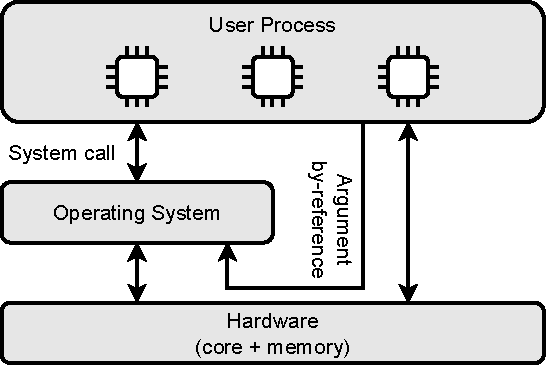
\includegraphics[width=0.6\linewidth]{media/midas_summary.pdf}
      \caption[Illustrating the double-fetch attack at the system call interface]
              {Illustrating the double-fetch attack at the system call interface}
      \label{fig:intro:midas}
\end{figure}

    
% Context
% \begin{itemize}
%   \item The design of many modern operating system kernels heavily draw inspiration from UNIX.
%         These kernels have progressively developed to incorporate modern features and modern
%         security models.
%   \item System call interfaces were designed in the era of uniprocessors.
%   \item Userspace was suspended during kernel syscall processing.
%   \item Multi-threading was not commonplace.
% \end{itemize}
The operating system (OS) kernel is a key component of modern computer systems,
tasked with multiplexing resources like memory, execution time and I/O among
users on a shared machine, or among different tasks by the same user.
The kernel is part of the system's trusted computing base (TCB), and interacts
with untrusted userspace processes through system calls (syscalls).
The userspace/kernel interface is a security-critical barrier, and forms the
primary attack vector for attacker processes to compromise an entire system.
The kernel must, therefore, implement extensive checks at this interface to
protect itself from malicious arguments to syscalls.
Most modern OS kernels trace their heritage to systems designed or developed in
the 1980's and 90's, and inherit many of their system calls.
The Linux, Darwin/XNU (used by MacOS) and FreeBSD kernels are all 
mostly compatible with the POSIX interface, first defined in 
1988~\cite{AtlidakisAGMN16}.
The POSIX interface, itself, draws inspiration from the UNIX kernel first
published in 1971.
Over this time, the computing landscape has evolved immensely.
Whereas the original UNIX kernel was not designed for multi-tasking, the
modern desktop, server or mobile computing environment involves a 
multi-user, multi-tasking, multi-processing systems connected via internal
or internet interfaces.
Kernel security has come under ever-increasing threats, and requires stronger
protection guarantees.
% CHATGPT version:
% The kernel of an operating system (OS) constitutes a pivotal element within
% contemporary computer systems, assigned the critical task of resource 
% multiplexing, including memory, execution time, and I/O distribution among 
% users sharing a common machine or among diverse tasks initiated by the same user. 
% As an integral component of the system's trusted computing base (TCB), the kernel 
% engages with untrusted userspace processes through system calls (syscalls). 
% The interface between userspace and the kernel emerges as a security-critical 
% boundary, representing the primary avenue through which malicious processes may 
% compromise the entire system. 
% Consequently, the kernel must implement rigorous checks at this interface to 
% safeguard itself against potentially malicious arguments passed through syscalls. 
% The lineage of most contemporary OS kernels can be traced back to systems 
% conceived or developed during the 1980s and 1990s. 
% Noteworthy among these are the Linux, Darwin/XNU (utilized by MacOS), and 
% FreeBSD kernels, all predominantly adhering to the POSIX interface, initially
% formalized in 1988. 
% The POSIX interface itself draws inspiration from the UNIX kernel, first 
% documented in 1971. 
% Across this temporal expanse, the landscape of computing has undergone 
% profound transformation. 
% While the original UNIX kernel lacked provisions for multitasking, the 
% present-day computing milieu encompasses multi-user, multitasking, and 
% multiprocessing systems interconnected through internal or internet 
% interfaces, spanning desktops, servers, and mobile platforms. 
% The escalating threats to kernel security necessitate heightened protection 
% guarantees. 
% As computing environments become more intricate and interconnected, the 
% imperative to fortify kernel security intensifies, underscoring the 
% exigency for robust defensive measures.


% Short introduction on the Kernel TOCTOTU problem.
% \begin{itemize}
%       \item User space uses system calls to request operating system kernel operations
%       \item System call arguments are passed through registers and through memory
%       \item Kernel reads userspace memory, sometimes in separate accesses for checks
%             and use (TOCTTOU)
%       \item Concurrent or parallel userspace threads sharing the address space can 
%             modify the arguments in memory
%       \item Earlier kernel code implicitly assumes that userspace is paused while
%             syscall executes. This assumption would be almost certain in less
%             adversarial environments, and on single-core computers.
%       \item Today, the kernel works with different threat assumptions, however, 
%             vulnerable code still remains, despite efforts to eliminate TOCTTOU.
%             Partly due to implicit assumptions
%             by developers, sometimes due to legacy code.
% \end{itemize}
Untrusted userspace processes interact with the kernel using system calls,
passing arguments by value (through registers) or by reference (in memory),
as illustrated in \autoref{fig:intro:midas}.
When an argument is passed by reference, and the kernel loads the same
value twice, an attacking user process can leverage the temporal window 
between the loads to modify the value in memory, potentially triggering a
kernel bug.
Double-fetch bugs plague operating system kernels, but also extend beyond
to the similar OS-hypervisor interface~\cite{cve201812633, cve202012652, 
cve20131332, cve201920610,cve20158550, cve201610439, cve201610435, 
cve201610433, cve20195519,cve20168438}.
For example, the user could pass a buffer, and its corresponding length
as arguments, then later maliciously change the length to influence the
kernel to access memory outside the buffer.
A time-of-check to time-of-use (\tocttou) violation occurs when the
first read is used to validate an argument (example, the length above)
and the second read is to use the argument.
More generally, a double-fetch bug manifests as system call code which reads
the same argument (passed by a user application by reference) two or more
times.
Double-fetch bugs might be particularly difficult to identify, as the two
reads might be in entirely different parts of the kernel, or even in external
code loaded through the eBPF interface or as modules.
Additional kernel security, such as through system call filters like 
SecComp~\cite{seccomp}, could also introduce double-fetches if extended to
include ``deep argument inspection'' (i.e., arguments passed by reference).

% Insight and design/solution mixed together
A systematic mitigation for double-fetch bugs must guarantee that a system call
will always read the same argument values.
Therefore, the mitigation must prohibit or hide all 
concurrent changes to memory objects accessed by the kernel 
during the execution of a system call, 
including writes from threads in the same process, other processes, 
or from concurrently executing system calls.
The userspace memory access interface can be tasked with providing
the required guarantee for argument accesses.

%%%%%%%%%%%%%%%%%%%%%%%%%%%%%%%%%%%%%%%%%%%%%%%%%%%%%%%%%%%%%%%%%%%%%%%%%%%%%%%
%%%%%%% Deeper dive into userspace compartmentalization
%%%%%%%%%%%%%%%%%%%%%%%%%%%%%%%%%%%%%%%%%%%%%%%%%%%%%%%%%%%%%%%%%%%%%%%%%%%%%%%
\section{Intra-address Space Compartmentalization Overview}

\begin{figure}
      \centering
      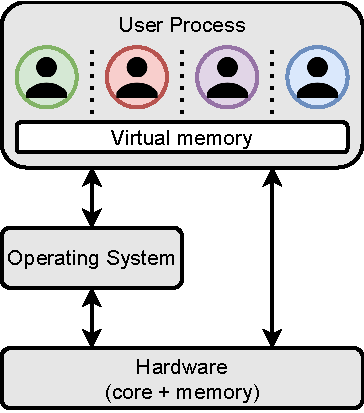
\includegraphics[width=0.4\linewidth]{media/seccells_summary.pdf}
      \caption[Illustrating intra-process trust components for an application]
              {Illustrating intra-process trust components for an application}
      \label{fig:intro:seccells}
\end{figure}

The complexity and rapid pace of change of modern software systems inevitably
leads to a plethora of bugs across the stack.
Open source projects regularly encounter and fix a steadily increasing stream
of bugs and vulnerabilities in their 
codebases~\cite{kernelbugs, browserwildbugs,vrprewards}.
System developers heavily rely on abstraction and isolation to tackle
application complexity stemming from interacting subsystems, 
an extensive list of shared libraries, 
plugins, interpreted code and on-demand downloaded code, interacting over 
untrusted I/O interfaces such as the network, disks, 
various accelerators, and peripherals.
Each software component hides much of its complexity behind an accessible
interface (commonly called Application Programming Interfaces or APIs).
Traditional threat models have resulted in isolation at a few 
security-critical interfaces.
The operating system (OS) kernel tasked with system management is already
isolated from userspace processes running untrusted applications.
Commercial hardware provides the abstraction of privilege levels, 
allowing the kernel to reliably isolate itself within a separate level.
The kernel isolates applications from different users and 
different applications from the same user using 
a common abstraction: processes.
Processes protect applications from other faulting or malicious applications,
with isolated per-process virtual memory spaces and kernel resources.
These abstractions provide systems crucial security and robustness 
guarantees.
Applications cannot access other applications' memory spaces, or the
kernel's data.
The kernel can gracefully handle an application faulting, killing the
corresponding process without affecting itself or other applications.
Essentially, these abstractions work to mirror the trust relations between
components of the massive code base.
However, existing interfaces fail to protect systems against more recent
threat models.

% Problem
Rapid development in computing, supercharged by the explosion of the internet,
has resulted in applications which cannot trust all code executing within
its process.
A bug in the one logging module allowed attackers to leverage the Log4J
vulnerability to compromise entire server applications, 
and remotely take over the machines running these applications.
A browser, for example, contains hundreds of shared libraries and executes
code downloaded from untrusted websites.
To prevent website code, controlled by a remote adversary, from directly 
accessing local resources, modern browsers are already compartmentalized into
two components: 
an internet-facing rendering engine running in one process 
interacting with 
a separate local system-facing kernel process
using a well-defined API over remote procedure calls (RPCs).
This architecture is motivated by the browser's strong security requirements,
but remains limited by the coarse-grained abstraction of isolation (processes)
available on traditional systems.
Bugs in the sandbox within the rendering engine can still compromise all
other components in the sandbox, including the just-in-time compiler.
The first key limitations of the process abstraction is that
all code within a process is equally privileged and 
can equally access all of that process' resources including memory.
The second limitation of this abstraction is that interactions between 
processes require system calls incurring microsecond-scale overheads.
The first limitation prevents applications from implementing and enforcing 
barriers expressing the complex trust relations between code components.
Applications rely on complex software isolation techniques like 
sandboxing and software fault isolation,
which are buggy at scale.
The second downside limits how finely applications can be decomposed into
processes, due to performance overhead considerations.
However, the process abstraction is flexible and widely supported, 
and remains the mechanism of choice for usable isolation.

% Insight and design/solution
Modern software requires an intra-address space compartmentalization mechanism
that provides strong isolation for application components
running within the same address space (see \autoref{fig:intro:seccells}), with
low-overhead nanosecond-scale operations to support compartments with short
nanosecond-scale execution timescales, all while maintaining the flexibility
to support a variety of software trust relationships.
In this thesis, we highlight that the limitations of the process abstraction
stem from the software-hardware design of virtual memory.
First, page-based virtual memory requires permission and translation tracking
at page granularity, and near-core permission caching buffers (TLBs) whose
entry count cannot scale with the rate of growth of memory.
Second, the privileged kernel is tasked with changing between memory 
permissions (involving changing page tables) and incurs the unacceptable
cost of kernel entry and exits.

% Describing solution methodology
Systems can implement secure and performant compartmentalization by moving
key checks and operations from the supervisor into the hardware.
While the hardware is part of the trusted-computing base, its view of virtual
memory remains rooted in the designs of the 80s.
A compartmentalized abstraction of virtual memory, with the hardware capable
of tracking compartments and enforcing the requisite permissions to memory,
can eliminate the kernel overheads while preserving strong security checks.
Further, the hardware can accelerate specific common compartmentalization
operations for data and control flow if it is aware of compartments.
Finally, operations which do not benefit from hardware acceleration can
be retained in software, retaining the accompanying flexibility.

%%%%%%%%%%%%%%%%%%%%%%%%%%%%%%%%%%%%%%%%%%%%%%%%%%%%%%%%%%%%%%%%%%%%%%%%%%%%%%%
%%%%%%% Zoom out, present the thesis statement
%%%%%%%%%%%%%%%%%%%%%%%%%%%%%%%%%%%%%%%%%%%%%%%%%%%%%%%%%%%%%%%%%%%%%%%%%%%%%%%
\section{Thesis Contributions}

This thesis aims to protect systems by redesigning interfaces to satisfy 
the security and performance requirements of modern and future computing 
systems, against emerging threat models.
While the security of current systems is of paramount importance, the
performance of these systems must also satisfy strict deployment 
requirements.
Foremost, we prioritize the security of our proposed interfaces, and
consider performance as a crucial secondary requirement.
For the user-kernel interface, we consider compatibility with
the existing system call semantics as an essential requirement.
For intra-address space compartmentalization, we  deem the flexibility
of the interface to support varying software use-cases to be vital for adoption.

% Summary of contributions
We present two redesigned security- and performance-critical 
interfaces, specifically the user-kernel boundary and 
intra-process trust domain boundaries.
We add strongly-guaranteed protection against double-fetch bugs to
the system call interface.
Further, we introduce a intra-address space mechanism for
isolating untrusted application parts.
Finally, we present a comprehensive survey of existing and proposed
compartmentalization mechanisms to enable a principled comparison
of these mechanisms.

\subsection{Midas}
Midas presents a multi-versioning concurrency control mechanism, inspired
from database systems, for maintaining a key invariant during user data
accesses from system calls:
\emph{through a system call's lifetime, every read to a userspace object
will return the same value}.
A \emph{security property} derived from this invariant is enforced ---
Midas uses kernel metadata to track userspace pages accessed, maintains
page-table permissions to enforce immutability and leverages page faults
to on-demand duplicate pages where necessary to preserve an original
copy for a system call.
A \emph{correctness property} is also described in this thesis,
showing how the system's execution remains correct under execution with
Midas.
Since, the user-kernel interface is performance-critical and 
affects the system's performance on syscall-intensive workloads,
Midas' design optimizes for low overheads.
As concurrent writes to system call arguments are practically non-existent
for well-behaved programs, Midas strives to minimize expensive page 
duplications and relies on snapshotting for protecting accesses.

Midas has numerous use cases.
First, Midas defends against existing, even potentially unknown,
double-fetch bugs on current and future systems.
Second, Midas can protect the kernel against double-fetch bugs in
dynamically-added code such as modules and eBPF code.
Third, Midas can enable system call filters to securely examine 
arguments passed by reference without introducing
vulnerable double-fetches.
Finally, Midas can protect older systems, where modules or other
vulnerable components lack bug-fixing updates, with a single update 
to the kernel core.

% Results summarized
We have implemented a Midas prototype for the Linux kernel, demonstrating its
practicality, and evaluated the system's performance during system-call
dependent workloads from the NAS Parallel Benchmark Suite (NPB) and the
Phoronix Test Suite (PTS).
Midas results in an average performance overhead of $3.7\%$ on NPB and
$3.4\%$ on PTS.
We also perform a security evaluation to demonstrate that Midas successfully
stops an attack against a vulnerable system call.

\subsection{SecureCells}
% What does SecureCells do and provide?
% SecureCells proposes a novel architecture, comprising
% \begin{itemize}
%   \item Compartmentalized virtual memory, with the hardware MMU responsible for
%         enforcing access control to memory across isolated compartments, based on 
%         per-core compartment identifiers and permissions stored on an in-memory
%         two dimensional table storing per-compartment, per-virtual memory permissions,
%   \item Userspace instructions, securely accelerating common compartmentalization 
%         operations implemented as hardware execution units, microcode or firmware,
%   \item Software operations, flexibly adding the remaining functionality with the
%         same security or performance guarantees as hardware.
% \end{itemize}
In this work, we also present a comprehensive set of objectives for a 
compartmentalization mechanism to support widespread adoption.
SecureCells presents a novel virtual memory architecture for secure, 
high-performance, flexible intra-address space compartmentalization.
SecureCells maintains the strong security guarantees of process-based isolation
for fine-grained compartments within a process, with a mix of hardware and
software support.
SecureCells tracks the compartment executing on a core, and implements access
control to memory regions based on a supervisor determined permission table
stored in memory.
Additionally, SecureCells provides unprivileged instructions to implement
fast compartmentalization operations, specifically inter-compartment calls,
zero-copy permission transfer to data regions, and to manage lifetimes for
data regions.
Each of these instructions includes specific checks and controls to maintain
specific security properties, including preventing privilege escalation,
code injection and data races.
Finally, SecureCells delegates operations to software when the corresponding
hardware implementation would bring no advantage.

% Implementation and results
This work also describes our prototype SecureCells implementation, including
the RTL description of an in-order core based on the RISC-V RocketChip design,
a QEMU port for quick emulation, porting of the seL4 microkernel operating
system, and simplified versions of server benchmarks.
We investigate the performance characteristics of our prototype core, using
microbenchmarks designed to test the limits of access control, compartment 
switching and dataflow between compartments, and compare them to related work.
SecureCells' in-order core can switch between compartments (a key performance
metric) in as few as 8 cycles, which compares favorably to state-of-the-art
compartmentalization mechanisms and is orders of magnitude faster than the
traditional process abstraction.
We also demonstrate that SecureCells can help isolate the networking and
data storage of a \Code{memcached}-like benchmark with a small ($<3\%$)
overhead even for the smallest requests.
These improvements are a direct consequence of tailoring the software-hardware
interface to the requirements of modern programs.

\begin{thesis}{Thesis statement}
      Critical interfaces underlying computing systems must adapt 
      to support mitigating emerging threats and 
      to enable the performance demanded by modern applications.
      Interfaces at key trust boundaries, e.g.,
      between untrusted intra-process components and 
      at the kernel-userspace border, 
      especially require strong isolation at low overheads.
\end{thesis}


%%%%%%%%%%%%%%%%%%%%%%%%%%%%%%%%%%%%%%%%%%%%%%%%%%%%%%%%%%%%%%%%%%%%%%%%%%%%%%%
%%%%%%% Thesis Outline
%%%%%%%%%%%%%%%%%%%%%%%%%%%%%%%%%%%%%%%%%%%%%%%%%%%%%%%%%%%%%%%%%%%%%%%%%%%%%%%
\section{Thesis Organization and Details}

\paragraph{Thesis Organization}
This thesis is distributed across three chapters. 
\autoref{ch:midas} describes Midas, the systematic mitigation to
kernel double-fetch bugs.
\autoref{ch:seccells} describes SecureCells, a novel secure and performant 
mechanism for intra-address space compartmentalization.
Finally, \autoref{ch:compsok} contains a comprehensive comparison of
compartmentalization mechanisms along qualitative and quantitative metrics.

%%%%%%%%%%%%%%%%%%%%%%%%%%%%%%%%%%%%%%%%%%%%%%%%%%%%%%%%%%%%%%%%%%%%%%%%%%%%%%%
%%%%%%% Reference the included papers and contributors
%%%%%%%%%%%%%%%%%%%%%%%%%%%%%%%%%%%%%%%%%%%%%%%%%%%%%%%%%%%%%%%%%%%%%%%%%%%%%%%
\paragraph{Bibliographic Notes}
This thesis was supervised by my advisors, Prof. Mathias Payer and Prof. Babak Falsafi.
Sections of the thesis describe projects conducted in collaboration with academic peers, 
namely Uros Tesic, Florian Hofhammer, Yuanlong Li, Siddharth Gupta, and Andres Sanchez.
This thesis contains contributions from the following conference publications:
\begin{itemize}
      \item \fullcite{BhattacharyyaTP22}
      \item \fullcite{BhattacharyyaHLGSFP23}
\end{itemize}

During the course of his PhD studies, the author of this thesis also contributed to
other projects resulting in the publications listed below.
The results from these publications are not included in this thesis.
\begin{itemize}
      \item \fullcite{JosipovicBGI19}
      \item \fullcite{BhattacharyyaSN19}
      \item \fullcite{BhattacharyyaSK20}
      \item \fullcite{0003BOBFP21midgard}
\end{itemize}